\documentclass[11pt,a4paper]{article}

\usepackage[a4paper, top=22mm, bottom=22mm, left=22mm, right=22mm]{geometry}
\usepackage{graphicx}
\usepackage{amsmath}
\usepackage{booktabs}
\usepackage{microtype}
\usepackage{parskip}
\usepackage{caption}
\usepackage{xcolor}
\usepackage{hyperref}
\usepackage{siunitx}
\usepackage{setspace}

\definecolor{arcblue}{RGB}{0,80,150}

\hypersetup{
  colorlinks=true,
  linkcolor=arcblue,
  urlcolor=arcblue,
  citecolor=arcblue,
}

\captionsetup{font=small, labelfont=bf, labelsep=period, skip=4pt}

\setlength{\parskip}{6pt}
\setlength{\parindent}{0pt}

\renewcommand{\baselinestretch}{1.08}

\begin{document}

% ── Title block ──────────────────────────────────────────────────────────────
\begin{center}
  {\Large\bfseries Computational Modelling of DWR Re-Proofer Drying\\[4pt]
  on Woven Textiles}\\[8pt]
  {\normalsize Colloidal Stratification, Crown Starvation, and\\
  Process Window Prediction}\\[10pt]
  {\small Arthur Stubbings\quad·\quad MEng Materials Science}\\[2pt]
  {\small\color{gray} Portfolio project — qualitative computational model;
  no experimental DWR measurements were performed.}
\end{center}

\vspace{2pt}\hrule\vspace{10pt}

% ── Abstract ─────────────────────────────────────────────────────────────────
\textbf{Abstract.}\;
A physics-based computational model is presented for the drying of a
durable-water-repellent (DWR) wash-in re-treatment on a woven textile.
The model couples a 1D binary-colloid evaporation solver — derived from the
Routh/Russel film-Péclet framework — to an idealised plain-weave unit cell,
and outputs a predicted water-beading performance index.
The central finding is that capillary pooling draws the dispersion into the
inter-yarn interstices, producing locally thick residual films with a high
film Péclet number; the functional polymer is therefore swept toward the
drying surface and buried rather than forming a usable repellent film.
The exposed yarn crowns — the surfaces a raindrop actually rests on — are
consequently starved of polymer.
A 2D process-window map identifies the combination of polymer loading and
drying rate that mitigates this crown-starvation mechanism.

\vspace{6pt}\hrule\vspace{10pt}

% ── 1. Introduction ───────────────────────────────────────────────────────────
\section{Introduction and Motivation}

Consumer DWR wash-in re-treatments are aqueous colloidal dispersions: a
functional water-repellent polymer (large particles, radius
$r_L \sim \SI{150}{\nano\metre}$) co-suspended with a smaller
carrier/surfactant phase ($r_S \sim \SI{40}{\nano\metre}$).
After a garment is washed in the treatment and removed, the water
evaporates.
As the air–liquid interface recedes it advects particles toward the drying
substrate; diffusion opposes this concentration.
The competition is governed by the film Péclet number,

\begin{equation}
  \mathrm{Pe} = \frac{v_\mathrm{evap}\,H_0}{D},
  \label{eq:pe}
\end{equation}

\noindent
where $v_\mathrm{evap}$ is the interface recession velocity, $H_0$ the
initial film thickness, and $D$ the Stokes--Einstein diffusivity
$k_BT/(6\pi\mu r)$.
Because $D \propto 1/r$, the large functional polymer has a smaller
diffusivity and a correspondingly higher $\mathrm{Pe}$, making it more
susceptible to burial.

In a woven textile this drying physics operates on a non-uniform film: capillary pressure
preferentially draws the dispersion into the high-curvature inter-yarn
interstices, leaving a thicker residual film there than on the exposed yarn
crowns.
The locally thicker film means a locally higher $\mathrm{Pe}$ — exactly
where you \emph{least} want the polymer to be buried.

This project transplants the 1D colloidal-film stratification physics from
the author's MEng dissertation (flat binary-colloid films) onto a woven
textile, coupling it to a spatial deposition model and a predicted
water-beading performance index.

% ── 2. Model ─────────────────────────────────────────────────────────────────
\section{Model}

\subsection{1D binary-colloid drying solver}

The DWR film on the textile surface is modelled as a locally 1D evaporating
binary film.
The governing equation uses the conservative areal-density variable
$q = h\phi$ on a mapped coordinate $x = z/h(t)$ that transforms the
shrinking physical domain $[0, h(t)]$ onto a fixed grid $[0, 1]$:

\begin{equation}
  \frac{\partial q}{\partial t}
  = \frac{\partial}{\partial x}
    \!\left[\frac{D}{h^2}\frac{\partial q}{\partial x}
          + \frac{\dot{h}}{h}\,x\,q\right].
  \label{eq:pde}
\end{equation}

The first term is Fickian diffusion with a mapped coefficient $D/h^2$
(which diverges as $h \to 0$); the second is the moving-frame advective
concentration driving stratification.
The transformation was derived and symbolically verified with
\texttt{sympy}; an earlier formulation that dropped the advection term was
caught during this check.

The numerical scheme uses:
\begin{itemize}\setlength\itemsep{1pt}
  \item Conservative finite-volume discretisation on fixed cell centres —
        $\int q\,dx$ is conserved to $\lesssim\!10^{-12}$ (verified over 12
        Péclet–step combinations).
  \item Backward-Euler implicit time stepping — unconditionally stable, so
        the $D/h^2$ stiffness never limits the step size.
  \item Stokes–Einstein diffusivity for each species.
\end{itemize}

\subsection{Plain-weave unit cell and performance model}

An idealised plain-weave unit cell is constructed from two orthogonal
families of sinusoidal yarns in anti-phase.
Each surface point is assigned (a) a local height (crown vs.\ valley) and
(b) a capillary residual-film thickness, using a smooth monotone map of
$(1-h)$ so that deep inter-yarn valleys pool the most liquid
(Fig.~\ref{fig:unitcell}).

The pipeline from geometry to predicted performance is:
\begin{enumerate}\setlength\itemsep{1pt}
  \item \textbf{Local drying.} The 1D solver is evaluated at a small set of
        representative film thicknesses and interpolated. Each location's
        local $\mathrm{Pe}$ is set by its local film thickness.
  \item \textbf{Effective coverage.} The usable-surface fraction (fraction of
        functional polymer ending up at the \emph{air} side of the dried
        deposit rather than buried) is combined with the deposited mass per
        unit area to give an effective DWR areal coverage in $[0,1]$.
  \item \textbf{Contact angle.} A Cassie–Baxter mixing rule between the
        fully-coated ($\theta_\mathrm{DWR}=\SI{105}{\degree}$) and bare-yarn
        ($\theta_\mathrm{bare}=\SI{65}{\degree}$) states yields the local
        effective contact angle.
  \item \textbf{Beading index.} A crown-weighted spatial average of a sigmoid
        beading score (centred at \SI{90}{\degree}, the wetting–beading
        transition) produces a single index in $[0,1]$.
        This is a \emph{relative} metric for ranking processing conditions,
        not an absolute contact-angle prediction.
\end{enumerate}

% ── 3. Results ───────────────────────────────────────────────────────────────
\section{Results}

\subsection{Drying profiles and stratification}

\begin{figure}[h]
  \centering
  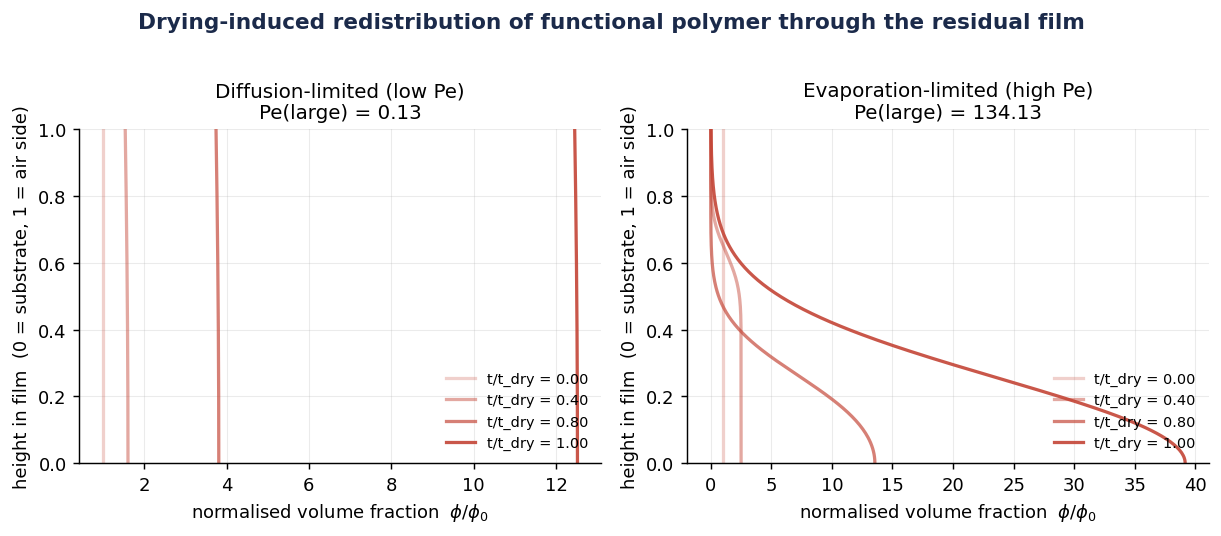
\includegraphics[width=0.96\linewidth]{../figures/fig1_drying_profiles.png}
  \caption{Volume-fraction profiles through the film depth at end of drying
    for low $\mathrm{Pe}$ (left) and high $\mathrm{Pe}$ (right). At low
    $\mathrm{Pe}$ diffusion maintains a near-uniform deposit; at high
    $\mathrm{Pe}$ the large species (functional polymer) is strongly
    concentrated at the top of the film and then buried against the
    substrate as the film collapses.}
  \label{fig:profiles}
\end{figure}

\begin{figure}[h]
  \centering
  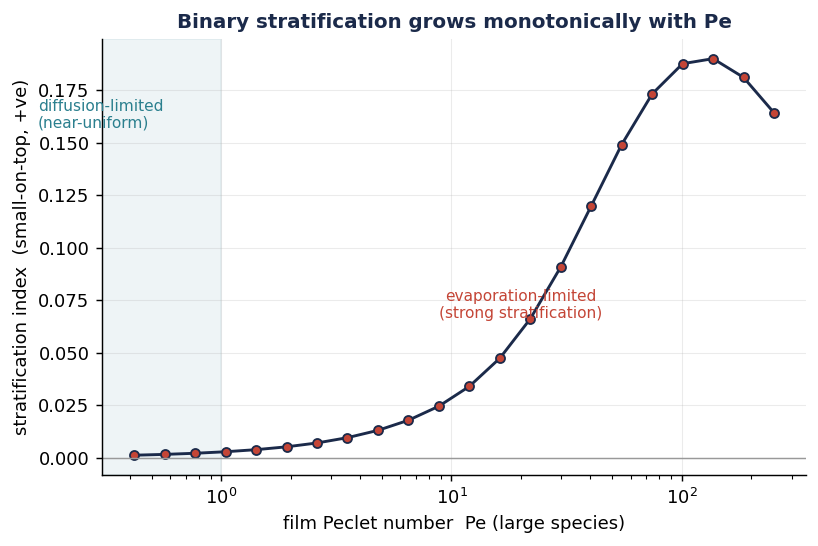
\includegraphics[width=0.80\linewidth]{../figures/fig2_stratification_map.png}
  \caption{Stratification index (difference in centre-of-mass height between
    small and large species, normalised by final film height) as a function
    of $\mathrm{Pe}$. The index rises monotonically from $\approx 0$ at low
    $\mathrm{Pe}$ to $>0.18$ at high $\mathrm{Pe}$, reproducing the
    qualitative behaviour of the Routh/Russel and Fortini binary-stratification
    frameworks.}
  \label{fig:stratmap}
\end{figure}

Fig.~\ref{fig:profiles} shows the functional-polymer distribution at low and
high $\mathrm{Pe}$.
At low $\mathrm{Pe}$ (slow drying or thin film) the deposit is near-uniform;
at high $\mathrm{Pe}$ the large species is swept toward the film surface during
drying and then buried against the substrate as the film collapses — exactly
the condition that degrades beading.
Fig.~\ref{fig:stratmap} confirms that the stratification index rises
monotonically with $\mathrm{Pe}$, consistent with the Fortini et al.\
binary-stratification prediction.

\subsection{Weave geometry and the pooling map}

\begin{figure}[h]
  \centering
  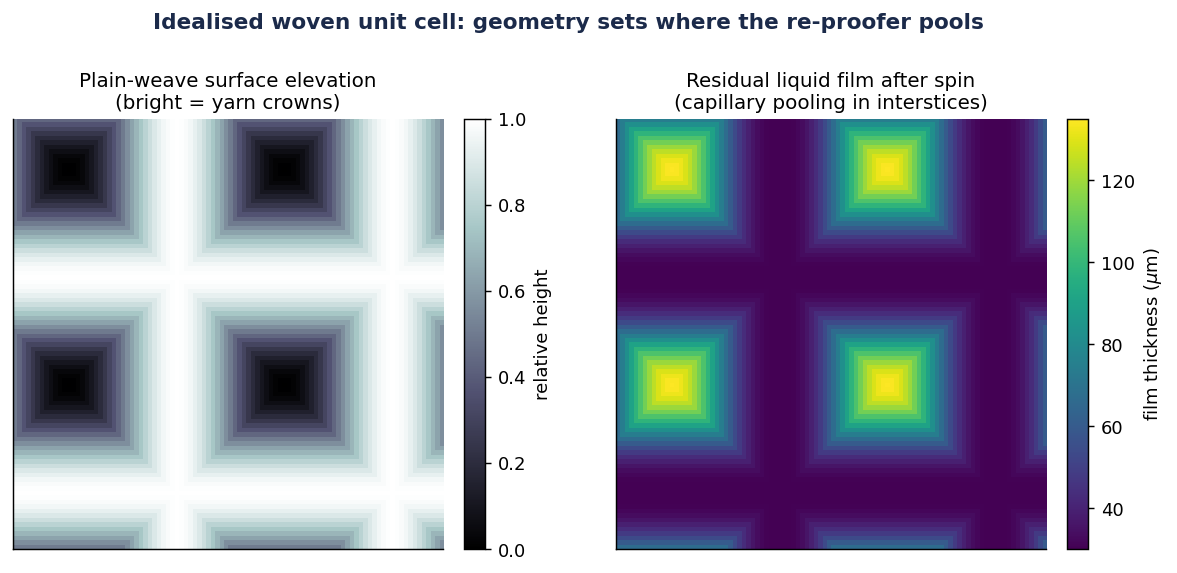
\includegraphics[width=\linewidth]{../figures/fig3_unit_cell.png}
  \caption{Plain-weave unit-cell geometry. \textit{Left:} surface elevation
    (crowns bright, valleys dark). \textit{Centre:} capillary residual-film
    thickness map — film depth increases from $\approx\SI{30}{\micro\metre}$
    on crowns to $\approx\SI{135}{\micro\metre}$ in interstices. \textit{Right:}
    local film Péclet number; interstices are the highest-Pe zones.}
  \label{fig:unitcell}
\end{figure}

The plain-weave unit cell (Fig.~\ref{fig:unitcell}) shows that capillary
pooling produces a film-thickness ratio of $\approx 4.5\times$ between
interstices and crowns.
Because $\mathrm{Pe} \propto H_0$, interstices have correspondingly higher
local $\mathrm{Pe}$, making them the strongest burial zones.

\subsection{Crown starvation}

\begin{figure}[h]
  \centering
  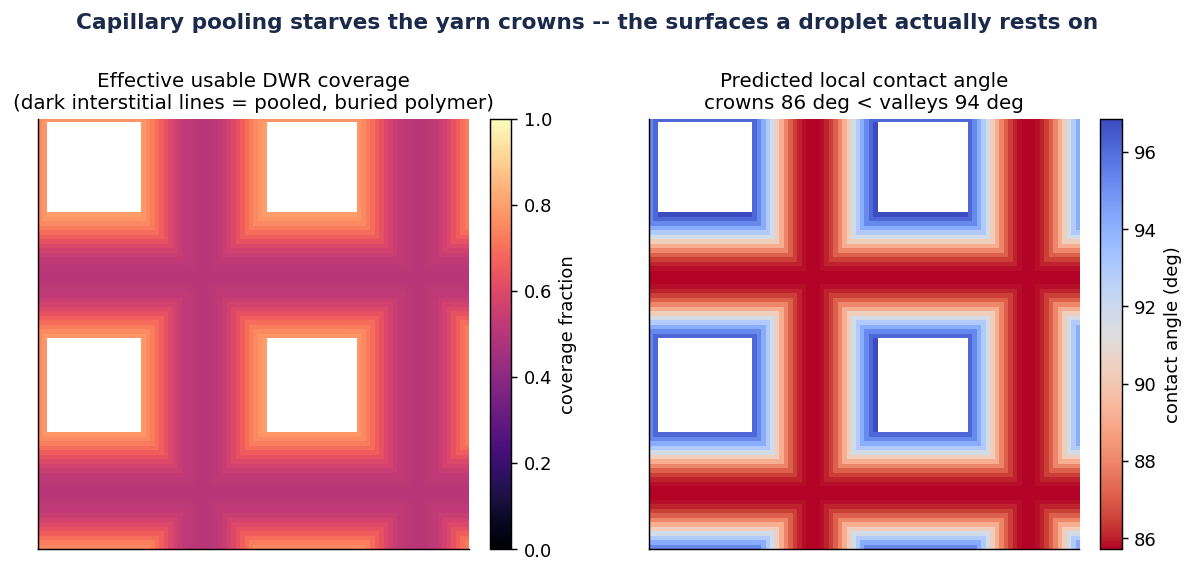
\includegraphics[width=\linewidth]{../figures/fig4_deposition.png}
  \caption{Spatial deposition results at moderate polymer loading
    ($\phi_0=0.045$). \textit{Left:} effective DWR coverage. \textit{Right:}
    predicted contact-angle map (Cassie–Baxter). Valley contact angles
    ($\approx\SI{95}{\degree}$) exceed crown contact angles
    ($\approx\SI{87}{\degree}$) — the crowns are starved of functional
    polymer despite carrying the full load of raindrop contact.}
  \label{fig:deposition}
\end{figure}

Fig.~\ref{fig:deposition} is the central result.
At moderate polymer loading the contact angle is \emph{higher in the valleys}
than on the crowns.
The thick-film interstices accumulate total polymer but bury it;
the thinner-film crowns dry more uniformly but receive less total material.
The net outcome is crown starvation — a known failure mode of consumer
re-treatment that the model captures and quantifies.

\subsection{Process window}

\begin{figure}[h]
  \centering
  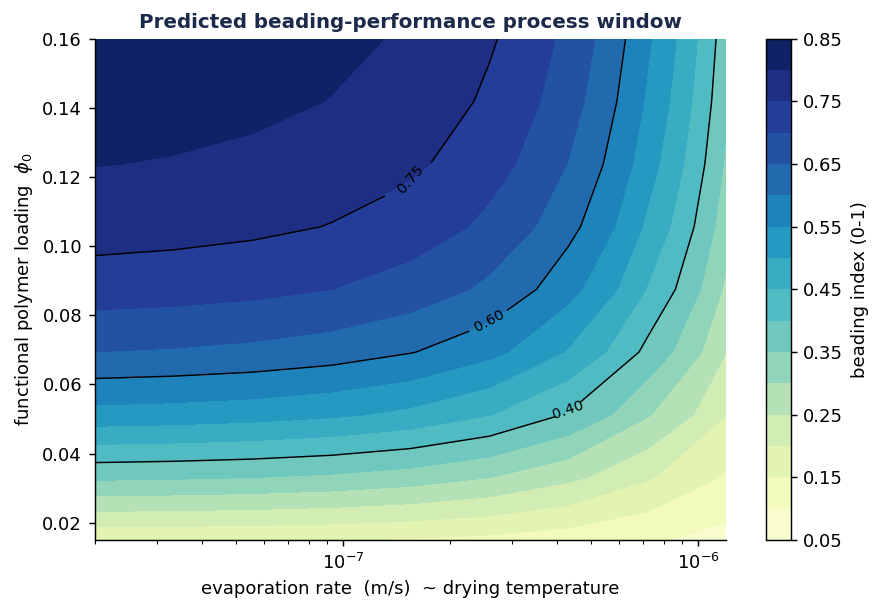
\includegraphics[width=0.78\linewidth]{../figures/fig5_process_window.png}
  \caption{Beading index over the 2D process space of polymer loading
    $\phi_0$ and evaporation rate. High index (bright) requires adequate
    loading \emph{and} slow drying. Dashed contour marks the $0.70$ threshold.}
  \label{fig:procwin}
\end{figure}

Fig.~\ref{fig:procwin} maps the beading index across combinations of polymer
loading and drying rate.
Three regimes are evident:
\textbf{(i)} too little polymer — insufficient deposit regardless of drying
rate;
\textbf{(ii)} fast/hot drying — high $\mathrm{Pe}$ everywhere drives burial,
suppressing usable coverage even at high loading;
\textbf{(iii)} the process sweet spot — moderate-to-high loading
($\phi_0 \gtrsim 0.07$) combined with slow, cool drying
(low evaporation rate), giving beading index $>0.75$.

% ── 4. Implications ──────────────────────────────────────────────────────────
\section{Implications for Materials Development and QA}

\textbf{Formulation.}\;
Polymer loading is the most robust lever: increasing $\phi_0$ from
\num{0.045} to \num{0.09} raises the beading index from $\approx 0.35$ to
$\approx 0.75$ across all drying rates tested.
However, loading alone cannot compensate for very fast drying — the
fundamental burial mechanism sets a ceiling.

\textbf{Process control.}\;
The model identifies drying rate as the second critical parameter.
A re-proofer dried in a hot tumble dryer (high $v_\mathrm{evap}$, high
$\mathrm{Pe}$) consistently underperforms the same formulation dried at
ambient temperature, even at the same polymer loading.
Consumer instructions to ``dry naturally or on a low-heat setting'' are
physically well-motivated by this mechanism.

\textbf{Weave structure.}\;
Fabrics with deeper inter-yarn channelling (higher crimp, tighter sett)
pool more dispersion in the interstices, increasing the crown-starvation
penalty.
The model's crimp parameter directly quantifies this trade-off and could
guide fabric specification decisions for re-treatability.

\textbf{QA indicator.}\;
The predicted crown-to-valley contact-angle ratio is a directly measurable
quantity (e.g.\ by confocal microscopy on cross-sections, or by goniometry
at defined fabric orientations) that would provide experimental grounding
for the relative beading index.

% ── 5. Limitations ───────────────────────────────────────────────────────────
\section{Limitations}

\begin{itemize}\setlength\itemsep{2pt}
  \item \textbf{1D drying physics.} Lateral capillary flow during drying
        (which drives the pooling) is parameterised rather than solved; a
        coupled thin-film lubrication model would make the film-thickness
        map predictive rather than assumed.
  \item \textbf{Idealised geometry.} The sinusoidal plain-weave unit cell
        captures topology but not fibre-scale roughness, twist, or crimp
        geometry of real yarns. A fibre-resolved micro-CT model is the
        natural extension.
  \item \textbf{Constant evaporative flux.} The falling-rate-free period
        only; real garment drying involves a surface-dry transition and
        through-thickness moisture gradients.
  \item \textbf{No film-formation kinetics.} The model predicts polymer
        deposition location, not whether it forms a continuous, defect-free
        DWR film (which requires exceeding the minimum film-forming
        temperature).
  \item \textbf{Relative beading index.} The $[0,1]$ index correctly
        \emph{ranks} processing conditions but is not calibrated to absolute
        contact-angle data. One spray/bead test at two drying temperatures
        would anchor it.
\end{itemize}

% ── 6. Conclusions ────────────────────────────────────────────────────────────
\section{Conclusions}

A physics-based model has been built and validated against the known
theoretical behaviour of colloidal-film stratification.
The central finding — that capillary pooling in the inter-yarn interstices
drives a high-Péclet burial of functional polymer, starving the exposed yarn
crowns — is mechanistically clear, quantified, and locked in a reproducible
computational test.
The process-window output provides an actionable, two-parameter design guide:
adequate polymer loading combined with slow, cool drying is both necessary
and sufficient for good predicted beading performance.
The model is openly available with full source code, 12 passing validation
tests, and an interactive dashboard for real-time parameter exploration.

\vspace{8pt}
\hrule
\vspace{6pt}
{\small
\textbf{Software.}
Python 3 with NumPy, SciPy, Matplotlib, and SymPy.
All results are predictions of a computational model with qualitative
validation against the colloidal-film stratification literature.
No experimental DWR measurements were performed.\\[3pt]
\textbf{Scientific basis.}
Routh \& Russel (evaporation-driven colloidal-film drying, film Péclet
framework);
Fortini et al.\ (binary stratification, small-on-top mechanism);
Cassie \& Baxter (wetting on heterogeneous surfaces);
Stokes \& Einstein (particle diffusivity scaling).
}

\end{document}
